%%
%% Meta: TI nSpire Einführung
%%       Ziel: Damit die Grundoperationen damit durchgeführt werden können.
%%             Damit man sich an den Rechner gewöhnt.
%%

\input{bmsLayoutPage}

%%%%%%%%%%%%%%%%%%%%%%%%%%%%%%%%%%%%%%%%%%%%%%%%%%%%%%%%%%%%%%%%%%

\usepackage{amssymb} %% für \blacktriangleright
\renewcommand{\metaHeaderLine}{Funktionsbegriff}
\renewcommand{\arbeitsblattTitel}{\metaHeaderLine{} Arbeitsblatt (V 1.1)}

\begin{document}%%
\arbeitsblattHeader{}

\section{Aufgaben Funktionsbegriff}

\subsection{Funktionen?}
Bei welchen der folgenden Zuordnungen handelt es sich um Funktionen im
mathematischen Sinne?

Links: Definitionsbereich; Rechts: Wertevorrat


a) \noTRAINER{\bbwCenterGraphic{70mm}{img/FctA.png}} \TRAINER{Ja}

b) \noTRAINER{\bbwCenterGraphic{70mm}{img/FctB.png}} \TRAINER{Nein, von «B» darf
nur eine Zuordnug ausgehen.}

c) \noTRAINER{\bbwCenterGraphic{70mm}{img/FctC.png}} \TRAINER{Ja, es müssen nicht
alle Werte im Wertevorrat getroffen werden. Der Wertebereich ist hier
einfach die Zahl «1».}

d) \noTRAINER{\bbwCenterGraphic{70mm}{img/FctD.png}} \TRAINER{Nein, auch von «C»
im Definitionsbereich muss eine Zuordnung stattfinden.}

e) \noTRAINER{\bbwCenterGraphic{70mm}{img/FctE.png}} \TRAINER{Ja, denn der
Wertevorrat muss nicht erschöpft werden; analog Teilaufgabe c).}
%%
\noTRAINER{\newpage}%%
%%
\subsection{Funktionsvorschrift}
Für welche der folgenden Graphen gibt es eine Funktionsvorschrift im
mathematischen Sinne?

$$x\mapsto y = f(x)$$

\begin{tabular}{|p{80mm}|p{80mm}|}\hline
a) \noTRAINER{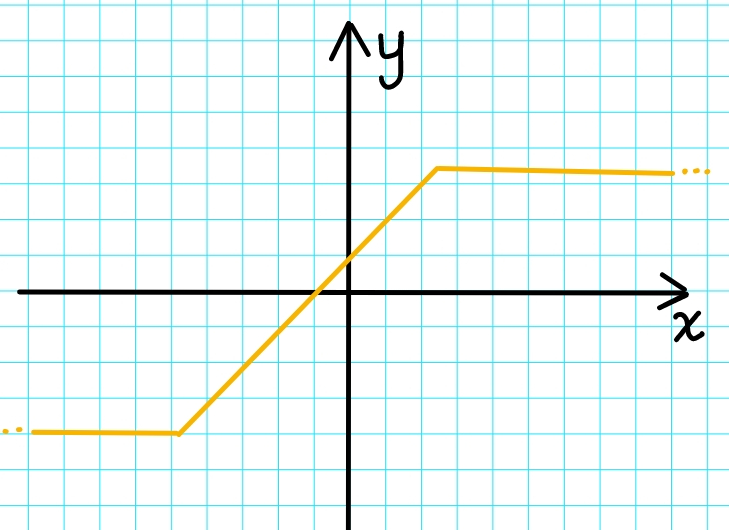
\includegraphics[width=60mm]{img/GraphA.jpg}}\TRAINER{ist Funktion} &
b) \noTRAINER{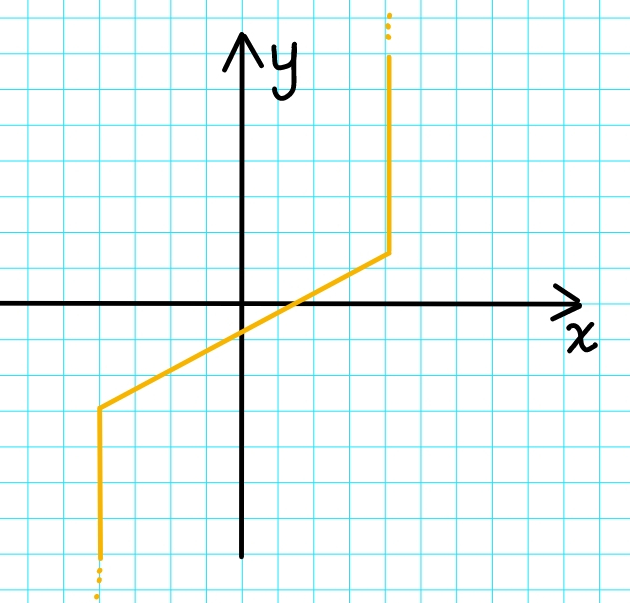
\includegraphics[width=60mm]{img/GraphB.jpg}}\TRAINER{keine Funktion}\\\hline
c) \noTRAINER{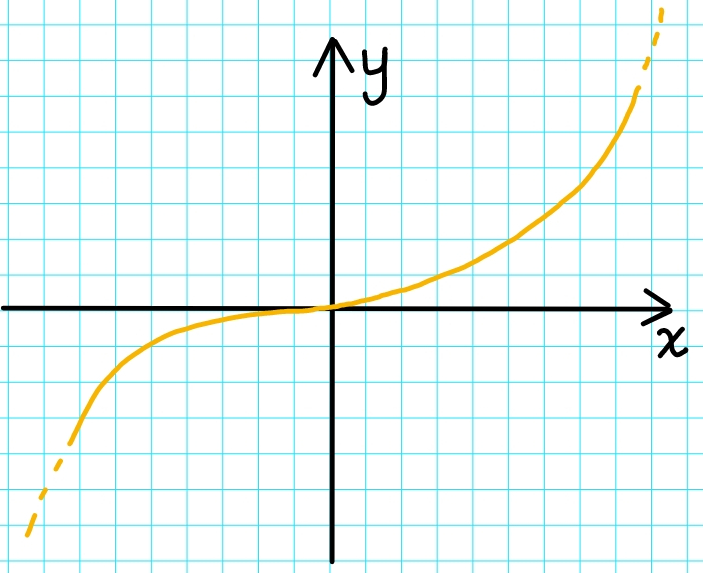
\includegraphics[width=60mm]{img/GraphC.jpg}}\TRAINER{ist Funktion} &
d) \noTRAINER{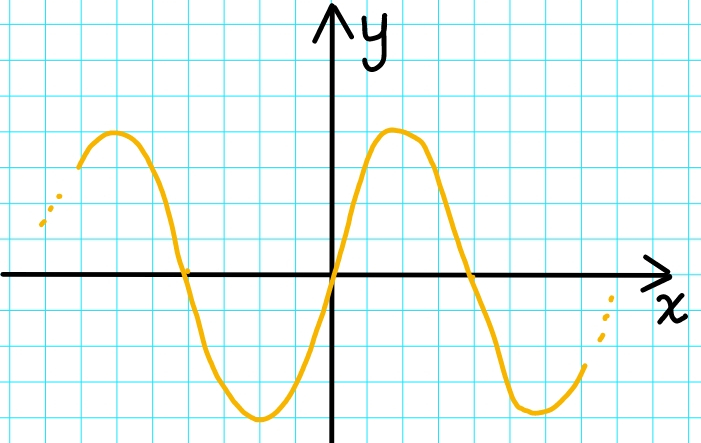
\includegraphics[width=60mm]{img/GraphD.jpg}}\TRAINER{ist Funktion}\\\hline
e) \noTRAINER{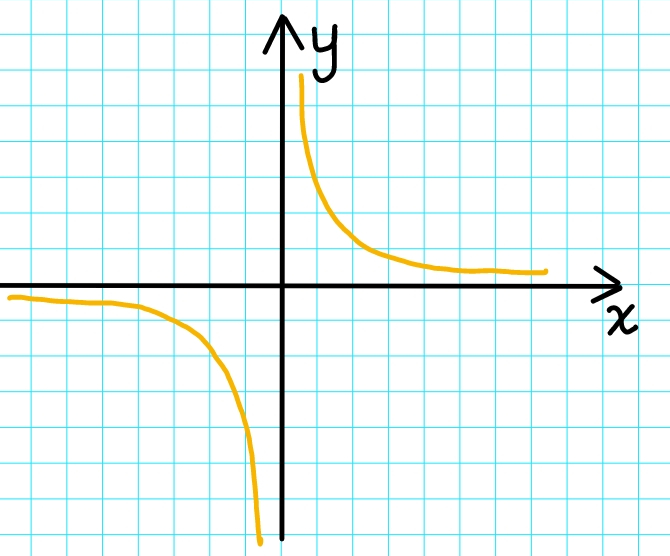
\includegraphics[width=60mm]{img/GraphE.jpg}}\TRAINER{ist
Funktion im Definitionsbereich $\mathbb{R}\backslash\{0\}$. Ansonsten
keine Funktion} &
f) \noTRAINER{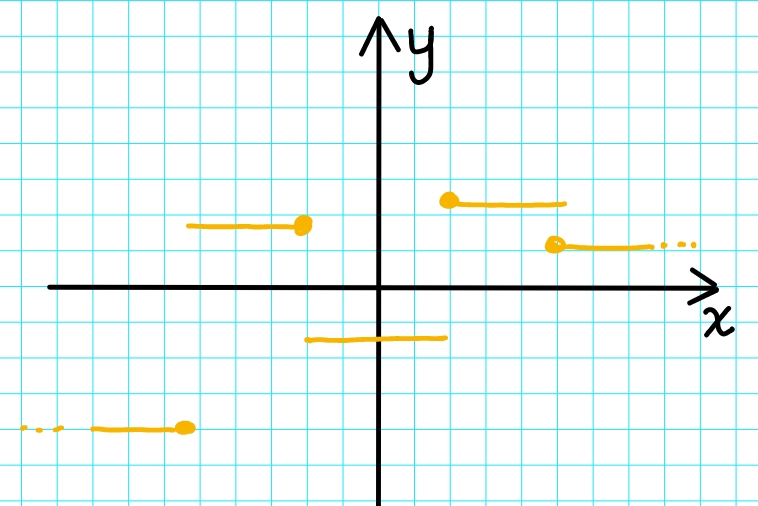
\includegraphics[width=60mm]{img/GraphF.jpg}}\TRAINER{ja
Funktion. Mit den «Punkten» am Ende der Strecken wird jeweils angegeben, welches der gültige
Funktionswert ist}\\\hline
g) \noTRAINER{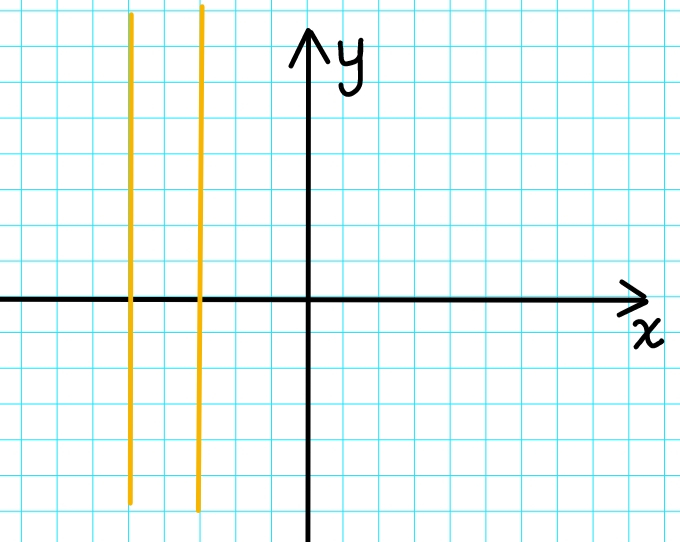
\includegraphics[width=60mm]{img/GraphG.jpg}}\TRAINER{keine Funktion} &
h) \noTRAINER{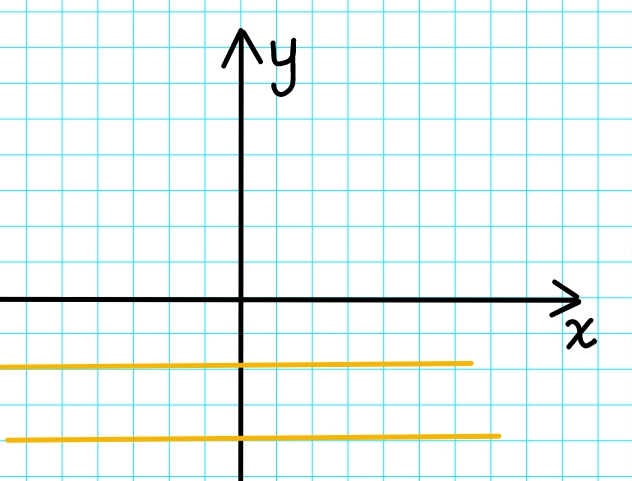
\includegraphics[width=60mm]{img/GraphH.jpg}}\TRAINER{keine Funktion}\\\hline
 \end{tabular}

%%
\newpage%%
%%
\subsection{Begriffe}
Gegeben ist $$f: y=\frac1{x^2} \text{ m. a. W. }
x\mapsto \frac1{x^2}$$
Ordnen Sie die Begriffe zu:

\noTRAINER{%%
\begin{tabular}{|rcl|}

Funktionsname        $\bullet$ & \hspace{40mm} & $\bullet$ $\frac1{x^2}$\\
Definitionsbereich   $\bullet$ & \hspace{40mm} & $\bullet$ $x$\\
Funktionsvorschrift  $\bullet$ & \hspace{40mm} & $\bullet$ $\mathbb{R}\backslash\{0\}$\\
Funktionsterm        $\bullet$ & \hspace{40mm} & $\bullet$ $\mathbb{R}$\\
unabhängige Variable $\bullet$ & \hspace{40mm} & $\bullet$ $\mathbb{R}^{+}\backslash\{0\}$\\
Wertevorrat          $\bullet$ & \hspace{40mm} & $\bullet$ $f$\\
abhängige Variable   $\bullet$ & \hspace{40mm} & $\bullet$ $y=\frac{1}{x^2}$\\
Funktionsgleichung   $\bullet$ & \hspace{40mm} & $\bullet$ $x\mapsto \frac{1}{x^2}$\\
Wertebereich         $\bullet$ & \hspace{40mm} & $\bullet$ $y$\\


\end{tabular}
}%% end noTRAINER
\TRAINER{\bbwCenterGraphic{150mm}{img/ZuordnungLoesung.png}}
\newpage


\subsection{Graphen}
Zeichnen Sie die Graphen der folgenden Funktionen und geben Sie
jeweils Definitionsbereich ($D$) und den Wertebereich($W$) an (Tipp: Wertetabelle):

a) $f(x) = (x+3)^2+1$

\bbwGraph{-5}{2}{-1}{5}{
\TRAINER{\bbwFunc{(\x+3)*(\x+3)+1}{-4.5:-1.5}}
}

$D = \LoesungsRaum{\mathbb{R};}$
\vspace{5mm}
$W = \LoesungsRaum{ \{     y\in\mathbb{R} | y \ge 1 \} }$
\vspace{5mm}

b) $g: y=\frac{x}2 - 1$

\bbwGraph{-4}{4}{-3}{1}{
\TRAINER{\bbwFunc{(\x / 2) - 1}{-3:3.5}}
}

$D = \LoesungsRaum{\mathbb{R}}$
\vspace{5mm}
$W = \LoesungsRaum{\mathbb{R}}$
\newpage
c) $h: x\mapsto \frac{1}{x-2}+3$

\bbwGraph{-4}{4}{-1}{5}{
\TRAINER{\bbwFunc{3+1/(\x-2)}{-3.5:1.8}}
\TRAINER{\bbwFunc{3+1/(\x-2)}{2.5:4}}
}

$D = \LoesungsRaum{\mathbb{R}\backslash{} \{2\}}$
\vspace{5mm}
$W = \LoesungsRaum{\mathbb{R}\backslash{} \{3\}}$
\newpage
\subsection{Funktion auswerten}
A: Werten Sie die folgende Funktion an den gegebenen $x$-Werten aus:

$$f: y = -x^2 + x$$

a) $x = 3$ \hspace{30mm} b) $x = \frac12$ \hspace{28mm} c)
$x=-1$ \hspace{26mm} d) $x=-\frac{-2}{-3}$

\vspace{5mm}

a) \LoesungsRaum{$-6$} \hspace{9mm} b) \LoesungsRaum{$\frac14$}\hspace{9mm}
c) \LoesungsRaum{-2} \hspace{9mm}d) \LoesungsRaum{$-\frac49 -\frac23 =
-\frac{10}9$}

\vspace{20mm}

B: Werten Sie die folgende Funktion an den gegebenen Argumenten aus:

$$s \mapsto \frac{-a}{s^2}$$

a) $s = 3$ \hspace{30mm} b) $s = -\frac12$

\vspace{5mm}
a) \LoesungsRaum{$-\frac{a}9$} \hspace{9mm}b) \LoesungsRaum{$-4a$}

\newpage
\subsection{«Umkehrfunktion»}
Gegeben ist die Funktion $f$:

$$f: y=(x-2)^2 + 3$$


a) Welches ist die unabhängige Variable?
\vspace{5mm}

Die unabhängige Variable ist $\LoesungsRaum{x}$.
\vspace{5mm}

b) Berechnen Sie den Funktionswert für das Argument $9$.
\vspace{5mm}

Der Funktionswert für das Argument neun ist $\LoesungsRaum{52}$.

\TRAINER{$$(9-2)^2+3 = 7^2 + 3 = 49 + 3 = 52$$}


c) Für welches Argument $x$ wird der Funktionswert zwölf getroffen?

$$\lx = \{\LoesungsRaum{-1}, \LoesungsRaum{5}\}$$

\TNTeop{
$$12     = f(x)$$
$$12     = (x-2)^2 + 3  | -3$$
$$9      = (x-2)^2     | \pm\sqrt{}$$
$$\pm 3  = x-2         | +2$$
$$2 \pm 3  = x         | +2$$
}
%%%%%%%%%%%%%%%%%%%%%%%%%%%%%%%%%%%%%%%%%%%%%%%%%%%%%%%%%%%%%%%555

\subsection{Relation prüfen}
Prüfen Sie für die Relation $$3x^2 + 2y^2 = 13$$ ob der Punkt $P$ auf
dem Graphen liegt:

a) $P=(2|2)$  \LoesungsRaum{$P$ liegt nicht auf dem Graphen}

\vspace{5mm}
b) $P=(1|-2)$  \LoesungsRaum{$P$ liegt nicht auf dem Graphen}

\vspace{5mm}
c) $P=\left(-\sqrt{\frac{5}{3}}\middle | -2\right)$  \LoesungsRaum{$P$ liegt auf dem Graphen}

\vspace{5mm}

\TNTeop{zu c)
$y=-2$ und $x = -\sqrt{\frac53}$ 
$$3x^2 + 2\cdot{}(-1)^2 \stackrel{?}{=} 13 $$
$$3\cdot{}\left(-\sqrt{\frac53}\right)^2 + 2\cdot{}(-2)^2 = $$
$$3\cdot{}\left(\sqrt{\frac53}\right)^2 + 8 = $$
$$3\cdot{}\frac53 + 8 = $$
$$5 + 8 = 13$$
}


\end{document}
